% capitoli/cap1.tex

\chapter{Introduzione teorica ai motori sincroni}
\label{chap:introduzione} % Etichetta per citare il capitolo altrove




\section{Procedura di misurazione}
L’equazione della tensione di statore è espressa nel sistema di riferimento rotante dq, sincrono rispetto al motore. \\
Come encoder si udìtilizza un encoder incrementale con 512 impulsi.
\section{Descrizione del progetto}
L'obiettivo del progetto di tesi è implementare una tecnica di stima flusso magnetico di un motore sincrono in funzione delle correnti d-q e della posizione.\\
Per verificare il funzionamento del sistema, si è implementato il modello su Simulink. 



\section{Motore IPM}
Il motore oggetto di studio è un motore IPM (Isochronous Permanent Magnet). I motori sincroni a magneti permanenti presentano un'anisotropia magnetica significativa dovuta alla struttura del motore e alla disposizione dei magneti permanenti.


\begin{figure}
    \centering
    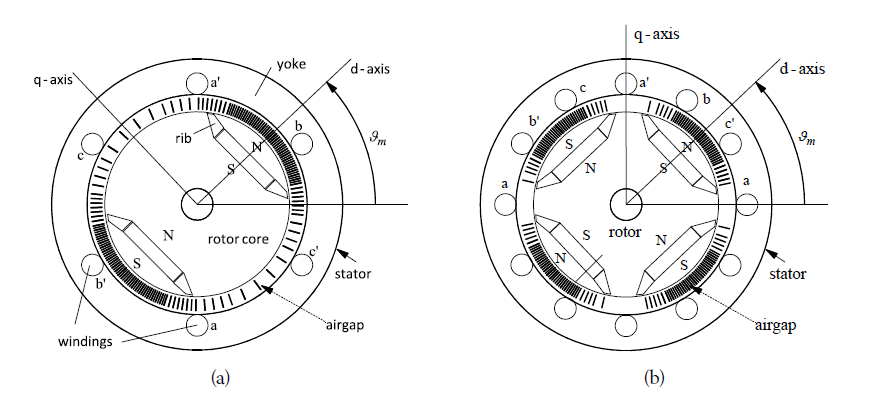
\includegraphics[width=1\linewidth]{immagini/immagini_motore/struttura_motore.png}
    \label{fig:Lez_10_5}
    \caption{Struttura del motore.}
\end{figure}

La distribuzione degli avvolgimenti di statore e la geometria dei magneti
permettono di ottenere flussi concatenati con il seguente andamento:

\begin{equation*}
\begin{aligned}
    &\lambda_{a,mg}=\Lambda_{mg}cos(\theta_{me})\\
     &\lambda_{b,mg}=\Lambda_{mg}cos(\theta_{me}-\frac{2}{3}\pi)\\
     &\lambda_{c,mg}=\Lambda_{mg}cos(\theta_{me}-\frac{4}{3}\pi)
    \end{aligned}\\
\end{equation*}
dove $\Lambda_{mg}$ rappresenta il massimo flusso concatenato dovuto al magnete permanente. Si può osservare come la terna di grandezze sia priva di componente omopolare; tale terna può quindi essere rappresentata tramite un unico vettore spaziale:

\begin{equation}
    \lambda_{mg}^s=\Lambda_{mg}e^{j\theta_{me}}
\end{equation}
 l’ apice $s$ indica che la grandezza è espressa secondo un sistema di riferimento stazionario,
 solidale con lo statore.  In tali motori la riluttanza lungo
l’ asse del loro campo magnetico (asse d) è maggiore rispetto a quella
secondo l’ asse ad essi ortogonale (asse q). L’ induzione magnetica è influenzata anche dal traferro e risulta dipendente anche della posizione del rotore. A differenza di altre tipologie di motore, le auto e mutue
induttanze non possono
essere considerate costanti, per la loro dipendenza dalla posizione del rotore e
dunque indirettamente anche dal tempo.\\
Le autoinduttanze del motore anisotropo si possono espriere nel modo seguente:
\begin{equation}
    \begin{aligned}
    &L_a=L_\sigma+L_0-L_2cos(2\theta_{me})\\
    &L_b=L_\sigma+L_0-L_2\cos{(2\theta_{me}-\frac{4}{3}\pi)}\\
    &L_c=L_\sigma+L_0-L_2\cos{(2\theta_{me}-\frac{2}{3}\pi})
    \end{aligned}
    \label{eq:inductances}
\end{equation}
dove indicando con $\Re_d$ ed $Re_q$ rispettivamente la riluttanza secondo l’asse d e
secondo l’asse q, e con N il numero “effttivo” di spire per fase, comprensivo di
ogni fattore necessario a correlare il numero di spire reali di un avvolgimento
distribuito con quello di un equivalente avvolgimento concentrato lungo ciascun
asse, si ha:

\begin{equation}
    L_0=N^2\frac{1/\Re_d+1/\Re_q}{2} \hspace{4mm} L_2=N^2\frac{1/\Re_d-1/\Re_q}{2} \hspace{4mm}
    \label{eq:double_L2}
\end{equation}
Come evidenziato dalla \ref{eq:inductances} le autoinduttanze si possono considerare somma
di due termini, uno sinusoidale a pulsazione doppia rispetto a quella elettromeccanica,
e l’altro costante. Quest’ultimo è formato a sua volta da due parti;
la prima, $L_0$, è legata ancora alla anisotropia della struttura, mentre la seconda,
$L_\sigma$ , rappresenta l’induttanza di dispersione ed è relativa al fluusso statorico che si
richiude in aria senza interessare il rotore.
Allo stesso modo, è possibile esprimere anche le mutue induttanze tra gli
avvolgimenti delle fasi statoriche, come segue:

\begin{equation}
\begin{aligned}
    & M_{ab}= \frac{1}{2}L_0-L_2\cos{\Big(2\theta_{me}-\frac{2\pi}{3}\Big)} \\
    & M_{bc}= \frac{1}{2}L_0-L_2\cos{(2\theta_{me})} \\
    & M_{ac}=-\frac{2}{2}L_0-L_2\cos{\Big(2\theta_{me}-\frac{4\pi}{3}\Big)}
\end{aligned}
\label{eq: equation4}
\end{equation}
dove $L_0$ ed $L_2$ rimangono  quelle definite dalle (\ref{eq: equation4}).\\
I flussi concatenati totali sono espressi dalla
\begin{equation}
\begin{aligned}
    & \lambda_a= L_ai_a+M_{ab}i_b+ M_{ac}i_c+ \lambda_{a,mg} \\
    & \lambda_a= L_bi_b+M_{ab}i_b+ M_{bc}i_c+ \lambda_{b,mg} \\
    & \lambda_a= L_ci_c+M_{ac}i_a+ M_{bc}i_b+ \lambda_{c,mg}
\end{aligned}
\label{eq: equation9}
\end{equation}
Le equazioni di bilancio delle tensioni sono:
\begin{equation}
\begin{aligned}
    & u_a= Ri_a+L_a\frac{di_a}{dt}+M_{ab}\frac{di_b}{dt}+M_{ac}\frac{di_c}{dt}+\frac{dL_a}{dt}i_a+\frac{dM_{ab}}{dt}i_b+\frac{dM_{ac}}{dt}i_c+e_a\\
    & u_b= Ri_b+L_b\frac{di_b}{dt}+M_{ab}\frac{di_a}{dt}+M_{bc}\frac{di_c}{dt}+\frac{dL_b}{dt}i_b+\frac{dM_{ab}}{dt}i_a+\frac{dM_{bc}}{dt}i_c+e_b \\
    & u_c= Ri_c+M_{ac}\frac{di_a}{dt}+M_{ab}\frac{di_a}{dt}+M_{bc}\frac{di_b}{dt}+\frac{dL_c}{dt}i_c+\frac{dM_{ac}}{dt}i_a+\frac{dM_{bc}}{dt}i_b+e_c \\
\end{aligned}
\label{eq: equation7}
\end{equation}
dove le forze contro-elettromotrici $e_a$,$e_b$, $e_c$ rimangono definite dalla
\begin{equation}
\begin{aligned}
    &e_a=\frac{d\lambda_{a,mg}}{dt}=-\Lambda_{mg}\omega_{me}sin(\theta_{me})\\
    &e_b=\frac{d\lambda_{b,mg}}{dt}=-\Lambda_{mg}\omega_{me}cos(\theta_{me}-\frac{\pi}{2}-\frac{2\pi}{3})\\
    &e_a=\frac{d\lambda_{a.mg}}{dt}=-\Lambda_{mg}\omega_{me}cos(\theta_{me}-\frac{\pi}{2}-\frac{4\pi}{3})\\
    \end{aligned}
\label{eq: equation5}
\end{equation}

Per comodità è utile esprimere le grandezze elettriche secondo il sistema di riferimento rotante. A tal scopo si impiega la seguente matrice di trasformazione di coordinate:

\begin{equation}
\mathbf{T_{abc/dq0}} = \frac{2}{3}
\begin{bmatrix}
    \cos (\vartheta_{me}) & \cos \left( \vartheta_{me} - \frac{2\pi}{3} \right) & \cos \left( \vartheta_{me} - \frac{4\pi}{3} \right) \\[6pt]
    -\sin (\vartheta_{me}) & -\sin \left( \vartheta_{me} - \frac{2\pi}{3} \right) & -\sin \left( \vartheta_{me} - \frac{4\pi}{3} \right) \\[6pt]
    \frac{1}{\sqrt{2}} & \frac{1}{\sqrt{2}} & \frac{1}{\sqrt{2}}
\end{bmatrix}
\label{eq:trasformazione_park}
\end{equation}
Le equazioni elettriche riportate \ref{eq: equation7}) possono essere espresse in maniera più compatta utilizzando una formulazione vettoriale:

\begin{equation}
\bm{u}_{abc}=\bm{Ri}_{abc}+\frac{d(\bm{L}_{abc}\bm{i}_{abc})}{dt}+\bm{e}_{abc}
\label{eq:equation10}
\end{equation}
dove le componenti vettoriali valgono:
\begin{align*}
\boldsymbol{u}_{abc} &= \begin{bmatrix} u_a & u_b & u_c \end{bmatrix} \\
\boldsymbol{i}_{abc} &= \begin{bmatrix} i_a & i_b & i_c \end{bmatrix} \\
\boldsymbol{e}_{abc} &= \begin{bmatrix} e_a & e_b & e_c \end{bmatrix}
\end{align*}
 le matrici $\bm{R}$ e $\bm{L_{abc}}$ sono definite come segue:
\begin{equation}
\bm{R} = 
\begin{bmatrix}
    R & 0 & 0 \\[6pt]
    0 & R & 0 \\[6pt]
    0 & 0 & R
\end{bmatrix}
\label{eq:trasformazione_park2}
\end{equation}

\begin{equation}
\bm{L}_{abc} = 
\begin{bmatrix}
    L_a & M_{ab} & M_{ac} \\[6pt]
    M_{ab} & L_b & M_{bc} \\[6pt]
    M_{ac} & M_{bc} & L_c
\end{bmatrix}
\label{eq:trasformazione_park3}
\end{equation}

Applicando alla (\ref{eq:equation10}) la trasformazione (\ref{eq:trasformazione_park}) si ottiene l’espressione matriciale
del bilancio delle tensioni nel sistema di riferimento sincrono, di seguito
riportata:
\begin{equation}
\mathbf{u}_{dq0}=\bm{Ri}_{dq0}+\bm{L}_{dq0}\frac{d\bm{i}_{dq0}}{dt}+\bm{e}_{abc}
\label{eq:electric_equa}
\end{equation}
dove
\begin{equation}
\begin{aligned}
\bm{u}_{dq0} &= [\, u_d \quad u_q \quad u_0 \;]' \\
\bm{i}_{dq0} &= [\, i_d \quad i_q \quad i_0 \,]
\end{aligned}
\label{eq:double_equa}
\end{equation}




ed inoltre, ricordando le (\ref{eq: equation5}):
\begin{equation}
    \bm{e}_{dq0}=[\,0\quad \omega_{me}\quad 0\,]'
\end{equation}
ed anche

\begin{align}
\bm{L}_{dq0} &=
\begin{bmatrix}
    L_d & 0 & 0 \\[6pt]
    0 & L_q & 0 \\[6pt]
    0 & 0 & L_\sigma
\end{bmatrix} \label{eq:trasformazione_park4} \\[12pt]
\bm{T} \frac{d\bm{T}^{-1}}{dt} &=
\begin{bmatrix}
    0 & -\omega_{me} & 0 \\[6pt]
    \omega_{me} & 0 & 0 \\[6pt]
    0 & 0 & 0
\end{bmatrix} \label{eq:trasformazione_park5}
\end{align}

come si può ricavare in maniera diretta applicando estesamente le formule di
Werner.\\
Le autoinduttanze $L_d$ e $L_q$ sono
legate ai termini $L_0$, $L_2$ ed $L_\sigma$ dalle relazioni:
\begin{equation}
L_d = L_\sigma + \frac{3}{2}(L_0 - L_2) \qquad L_q = L_\sigma + \frac{3}{2}(L_0 + L_2)    
\label{eq:double_L}
\end{equation}

Nei motori 
IPM la riluttanza del circuito magnetico associato all’asse $d$ è superiore a quella
relativa all’asse $q$ ne segue, dalle (\ref{eq:double_L2}) che $L_0$ ed $L_2$ siano entrambe positive, con
$L_0>L_2$; quanto scritto trova riscontro ovviamente anche nelle (\ref{eq:double_L}), ove
appare evidente che $L_q>L_d$. In particolare, il rapporto $L_q/L_d$ prende il nome
di rapporto di salienza e negli IPM può arrivarefino a 5.\\
Vale la pena di osservare che, in caso di rotore isotropo, verrebbe a mancare
il termine $L_2$. Si
preferisce l’impostazione attuale perché essa consente di arricchire di significato  fisico i vettori spaziali e, con essi, di dare una visione più intuitiva del principio
dell’orientamento di campo, che sta alla base degli azionamenti con motore
sincrono a magneti permanenti.\\
La relazione matriciale (\ref{eq:electric_equa}) può essere scritta tenendo conto delle (\ref{eq:double_equa})-(\ref{eq:trasformazione_park5})
per ciascuna delle sue tre componenti, ottenendo:

\begin{equation}
\begin{aligned}
    &u_d=Ri_d+L_d\frac{di_d}{dt}-\omega_{me}L_qi_q\\
    &u_q=Ri_q+L_q\frac{di_q}{dt}+\omega_{me}L_di_d+\omega_{me}\Lambda_{mg}\\
    &u_0=Ri_0+L_\sigma\frac{di_0}{dt}\\
    \end{aligned}
\label{eq: equation6}
\end{equation}
Le componenti della tensione secondo gli assi diretto ed in quadratura
hanno un’espressione sostanzialmente equivalente a quella ricavata per il motore
isotropo, quando in quest’ultima si sostituisca opportunamente all’induttanza
sincrona $L$ le induttanze sincrone d’asse diretto ed in quadratura.\\
Le espressioni (\ref{eq: equation6}) consentono di tracciare il bilancio energetico nel sistema
di riferimento sincrono, per ricavare un’espressione per la coppia meccanica
    sviluppata dal motore. In questo caso, si moltiplichino ambo i membri delle (\ref{eq: equation6}) rispettivamente per $i_ddt$, $i_qdtB$ e $i_odt$. Sommando membro a membro le tre
equazioni si ottiene:

\begin{equation}
\begin{aligned}
(u_d i_d + u_q i_q + u_0 i_0) dt &= R \left( i_d^2 + i_q^2 + i_0^2 \right) dt \\
&\quad + L_d i_d di_d + L_q i_q di_q + L_\sigma i_0 di_0 \\
&\quad + \omega_{me} \left( \Lambda_{mg} i_q + (L_d - L_q) i_d i_q \right) dt
\end{aligned}
\label{eq:bilancio_potenza}
\end{equation}

La coppia sviluppata dal motore risulta:
\begin{equation}
 \tau=\frac{3}{2}p\Lambda_{mg}i_q+\frac{3}{2}p(L_d-L_q)i_di_q
 \label{eq:equazione9}
\end{equation}

Rispetto al caso di motore isotropo si verifica la presenza di un ulteriore
termine, detto coppia di riluttanza.\\
Il contributo dovuto alla coppia di riluttanza accresce l’efficienza della conversione
elettromeccanica, intesa come rapporto tra coppia prodotta e modulo
(o valore massimo, a seconda del sistema di riferimento) della corrente di alimentazione.
I motori a magneti sepolti risultano dunque più economici di quelli a
magnete superficiale, perché è possibile impiegare meno materiale magnetico a
parità di coppia prodotta. La costruzione meccanica, che risulta intrinsecamente
robusta perché adatta a contrastare l’effetto della forza centrifuga sui magneti in
rotazione, e la possibilità di deflusare il motore in un range più esteso di quello
dei corrispondenti motori PMSM, rendono gli IPM adatti ad applicazioni ad
alte velocità ed alte prestazioni.\\
Nelle (\ref{eq: equation6}) appare anche l’equazione del bilancio della tensione $u_0$, che rappresenta
la tensione omopolare moltiplicata per un coefficiente di scala
$\sqrt{2}$. Tale
tensione insorge ad opera della corrente omopolare che normalmente è nulla
per l’assenza del filo neutro nella maggior parte dei motori sincroni a magneti
permanenti; come appare dalla (\ref{eq:equation10}) tale componente non partecipa alla creazione
della coppia e nello studio degli azionamenti per IPM verrà tralasciata.\\
In alcuni casi, come nelle moderne strategie di diagnosi dei guasti con adozione
automatica delle contromisure (fault-tolerant drives) vengono previsti
motori con il filo neutro, da collegare ad un quarto ramo dell’inverter che alimenta
il motore. Opportune tecniche di controllo provvedono poi ad isolare la
fase guasta e ad utilizzare il filo neutro come sua supplente; è nello studio di tali
tecniche avanzate che l’approccio generale presentato in questo paragrafo rivela
la sua utilità.\\
Dalle equazioni (\ref{eq: equation6}), (\ref{eq:equazione9}) e l’equazione che rappresenta il carico meccanico
si può infine tracciare lo schema a blocchi per il motore sincrono a magneti
permanenti di tipo anisotropo riportato nella Figura 2.
%______________________________________________________%

\section{Calcolo delle induttanza differenziali}
Le induttanze differenziali si possono ottenere calcolando le derivate parziali dei flussi:

\begin{equation}
\begin{dcases}
    \frac{d \lambda_d}{dt} = \frac{\partial \lambda_d}{\partial i_d} \frac{d i_d}{dt}+\frac{\partial \lambda_d}{\partial i_q} \frac{d i_q}{dt}+\frac{\partial \lambda_d}{\partial \theta_m} \frac{d \theta_m}{dt} \\[7pt] % <--- Aggiunge 15 punti di spazio
    \frac{d \lambda_q}{dt} = \frac{\partial \lambda_q}{\partial i_d} \frac{d i_d}{dt}+\frac{\partial \lambda_q}{\partial i_q} \frac{d i_q}{dt}+\frac{\partial \lambda_q}{\partial \theta_m} \frac{d \theta_m}{dt}
\end{dcases}
\end{equation}

Si può esprimere queste relazioni in maniera più compatta, usando il concetto di induttanze differenziali:

\begin{equation}
\begin{dcases}
    \frac{d \lambda_d}{dt} = l_d \frac{d i_d}{dt}+l_{dq} \frac{d i_q}{dt}+l_{d\theta} \frac{d \theta_m}{dt} \\[7pt] % <--- Aggiunge 15 punti di spazio
    \frac{d \lambda_q}{dt} = l_{qd} \frac{d i_d}{dt}+l_q \frac{d i_q}{dt}+l_{q\theta} \frac{d \theta_m}{dt}
\end{dcases}
\label{eq:induttanze_diff_elet}
\end{equation}

